%!TEX root = ../thesis.tex

\section{Introduction}\label{sec:introduction}

\todo[inline]{Expand}

Reconstructing character-based phylogenies, which are used to study the evolution of characters shared by a collection of species (taxa or individuals), is a recurring problem in Bioinformatics \todo{Citation needed}, mainly due to the complexity of the task \todo{Citation needed}. In fact, there exist multiple approaches to evolutionary history reconstruction \todo{Citation needed}; most of those approaches try to reduce the problem by limiting the way (or amount of times) characters can change state in the phylogenetic tree \cite{PPptime1994} \todo{Citation needed}. The Persistent Phylogeny model \todo{Citation needed}, which we will talk about in the following sections, allows characters to be acquired and lost at most once in the evolutionary history.

\subsection{Character evolution in Bioinformatics}\label{ssec:charevo}

\todo[inline]{Expand}

To study the state changes of characters in an evolutionary tree we can represent species and their characters as rows and columns of a matrix; each element of the matrix marks the specific state of a character for a species.

We will consider the case in which all characters are binary, making them able to assume only one of two states, 0 or 1. For each species, the state of a character represents if the species has or doesn't have a given feature.

Binary phylogeny models have already been explored \todo{Citation needed} and \dots

\begin{definition}\label{def:m}
  \m{} is a $n \times m$ binary matrix over a set $m$ of characters and a set $n$ of species.

  \m[i][j] represents the state of a character \character[j] for a species \species[i].
\end{definition}

A matrix \m{} can then be represented as an undirected bipartite graph. The set of vertices of the graph is $V = S \cup C$, where $S$ is the set of species and $C$ the set of characters.

\begin{figure}[h]
  %!TEX root = ../thesis.tex

\begin{subfigure}[b]{0.45\textwidth}
  \centering
    \begin{tabular}{c | c c c c}
      \m{}  & $c_0$ & $c_1$ & $c_2$ & $c_3$ \\ \hline
      $s_0$ & 0     & 1     & 1     & 1     \\
      $s_1$ & 0     & 0     & 0     & 1     \\
      $s_2$ & 1     & 1     & 0     & 0     \\
      $s_3$ & 1     & 0     & 1     & 0
    \end{tabular}

  \caption{Matrix for the instance}\label{figure:1:a}
\end{subfigure}
\hfill
\begin{subfigure}[b]{0.45\textwidth}
  \centering
    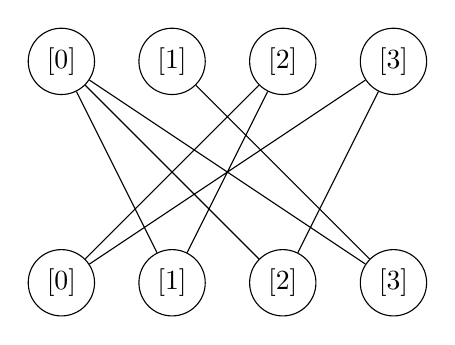
\begin{tikzpicture}
      {\tikzstyle{every node}=[circle, draw]
        \foreach \i in {0, ..., 3}
        {
          \node (s\i) at (\i*40pt, 80pt) {\species[\i]};
        }

        \foreach \j in {0, ..., 3}
        {
          \node (c\j) at (\j*40pt, 0) {\character[\j]};
        }
      }

      \draw
        (c0) -- (s2)
        (c0) -- (s3)
        (c1) -- (s0)
        (c1) -- (s2)
        (c2) -- (s0)
        (c2) -- (s3)
        (c3) -- (s0)
        (c3) -- (s1);
    \end{tikzpicture}

  \caption{Graph for the instance}\label{figure:1:b}
\end{subfigure}


  \caption{An instance of a character-based phylogeny represented as matrix and graph $(\text{4 species} \times \text{4 characters})$}
  \label{fig:1}
\end{figure}

In the figure above (\ref{fig:1}) we have a set of species $S = \{ \species[0], \species[1], \species[2], \species[3] \}$ and a set of characters $C = \{ \character[0], \character[1], \character[2], \character[3] \}$.
Each element $\m[i][j] = 1$ of the matrix (\ref{fig:1:a}) is shown as the edge \edge{\species[i]}{\character[j]} in the corresponding graph (\ref{fig:1:b}).

\subsubsection{Character states}\label{sssec:charstates}

\todo[inline]{Expand}

In a phylogenetic tree, characters can be acquired and lost; we will use the notation \character[][+] for acquired characters and \character[][-] for lost characters. Each \character[][+] and \character[][-] represents a \emph{signed} character.

The Persistent Phylogeny model enables characters to be lost at most once in the evolutionary events; we then need a way to keep track of the characters that were previously acquired. This is solved by introducing the concept of \emph{active} characters.

Active characters are a subset of the instance's current set of characters $C = \{ \character[0], \dots, \character[m-1] \}$.
A character becomes active whenever it is gained in the tree.

\subsection{Persistent Phylogeny problem}\label{ssec:ppp}

\wip[inline]{Expand}

A Persistent Phylogeny can also be called Persistent Perfect Phylogeny (P-PP, or simply put, PPP), since its model is directly related to that of the Perfect Phylogeny.

Each instance of a PPP is associated to a pair \ma{} and a rooted tree $T$, where $T$ is a \emph{persistent phylogeny} for the pair \ma{}. \fix{Reword? Too many repetitions} If \ma{} admits a persistent phylogeny we then say that the matrix $M$ is solved by the tree $T$ \cite{PPPptime2016,PPPcgraph2016}.

We now formalize input and output parameters for the Persistent Phylogeny problem \cite{PPPptime2016}.

\begin{definition}[Persistent Phylogeny problem]\label{def:ppp}
  \text{}

  \textit{Input:} pair \ma{} where \m{} is a $n \times m$ binary matrix over a set of $m$ characters and a set of $n$ species, and A is a subset of its characters.

  \textit{Output:} tree $T$ solving \m{} if it exists.
\end{definition}

\subsubsection{Red-black graph representation}\label{sssec:grb}

A red-black graph for an instance of PPP is an undirected bipartite graph whose edges are colored as either red or black.

\begin{definition}[Red-black graph for PPP]\label{def:grb}
  Let $S$ be a set of species vertices, $C$ a set of character vertices, $B$ a set of black edges and $R$ a set of red edges.
  Then \grb{} is defined as follows:

  \[ \grb{} = (S \cup C, B \cup R) \]

  The vertex set $V$ of \grb{} is formally represented as two disjoint and independent sets $S$ and $C$.

  The edge set $E$ of \grb{} is formally represented as two disjoint and independent sets $B$ and $R$.
\end{definition}

\todo[inline]{GRB and T are in relation thanks to the c-reduction}

A \emph{c-reduction} for a graph \grb{} is the sequence of operations that, when performed on an instance of PPP, clears the graph of all edges.
